%for testing sectioning purpose
% \section{Test thu}
% \input{chapters/sections/sections2.1}\\

\section{Microcontroller}
  \subsection{Theory}
  Microcontroller unit (MCU) is a small size, special purpose computer. It is small enough in order to be integrated on a small circuit in which will do specified tasks or applications. MCU itself comes with memory, input, output peripherals and processor. Program to run the MCU is stored in Read-only memory (ROM) and usually not change in production. A microcontroller is usually designed to run in small size and at low cost, which is compatible to be embedded in other system in order to control actions of the system automatically.

  \subsection{Microcontroller structure}
  
  \begin{figure}[h!]
    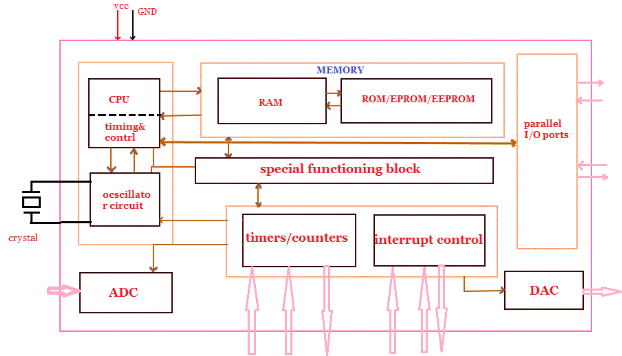
\includegraphics[scale=0.9]{images/Microcontroller-Structure.png}
    \caption{Structure of Microcontroller}
  \end{figure}
  


  \subsection{Microcontroller market}
  There exists many microcontrollers on the market which come in various sizes and capacities. The list is only contains very few popular MCU that the author knows of.
  \begin{itemize}
    \item Intel 8051
    \item STMicroelectronics STM8S (8-bit), ST10 (16-bit) and STM32 (32-bit)
    \item Atmel AVR (8-bit), AVR32 (32-bit), and AT91SAM (32-bit)
    \item Freescale ColdFire (32-bit) and S08 (8-bit)
    \item PIC (8-bit PIC16, PIC18, 16-bit dsPIC33 / PIC24)
    \item Renesas Electronics: RL78 16-bit MCU; RX 32-bit MCU; SuperH; V850 32-
    bit MCU; H8; R8C 16-bit MCU
    \item PSoC (Programmable System-on-Chip)
    \item Texas Instruments Microcontrollers MSP430 (16-bit), C2000 (32-bit), and
    Stellaris (32-bit)
  \end{itemize}

\section{Communication protocol}
  

